\documentclass{ctexart}
\usepackage{amsmath,amssymb,amsthm,bm}
\usepackage{xcolor}
\definecolor{Solarized-base03}{RGB}{0, 43, 54}
\definecolor{Solarized-base02}{RGB}{7, 54, 66}
\definecolor{Solarized-base01}{RGB}{88, 110, 117}
\definecolor{Solarized-base00}{RGB}{101, 123, 131}
\definecolor{Solarized-base0}{RGB}{131, 148, 150}
\definecolor{Solarized-base1}{RGB}{147, 161, 161}
\definecolor{Solarized-base2}{RGB}{238, 232, 213}
\definecolor{Solarized-base3}{RGB}{253, 246, 227}
\definecolor{Solarized-yellow}{RGB}{181, 137, 0}
\definecolor{Solarized-orange}{RGB}{203, 75, 22}
\definecolor{Solarized-red}{RGB}{220, 50, 47}
\definecolor{Solarized-magenta}{RGB}{211, 54, 130}
\definecolor{Solarized-violet}{RGB}{108, 113, 196}
\definecolor{Solarized-blue}{RGB}{38, 139, 210}
\definecolor{Solarized-cyan}{RGB}{42, 161, 152}
\definecolor{Solarized-green}{RGB}{133, 153, 0}
\color{Solarized-base01}
\pagecolor{Solarized-base3}

\newcommand{\red}[1]{\textcolor{Solarized-red}{#1}}
\newcommand{\yellow}[1]{\textcolor{Solarized-yellow}{#1}}
\newcommand{\blue}[1]{\textcolor{Solarized-blue}{#1}}
\newcommand{\cyan}[1]{\textcolor{Solarized-cyan}{#1}}
\newcommand{\violet}[1]{\textcolor{Solarized-violet}{#1}}

\usepackage{fullpage}
\usepackage{graphicx,epsfig,subfigure}
\usepackage{tikz,pgfplots}
\pgfplotsset{compat=1.17}
\usepackage{ifthen}
\usetikzlibrary{backgrounds,automata,shapes,snakes,arrows,arrows.meta,chains,positioning,calc}

%%%%%% 下面两行字体设置你们根据自己的系统调整
\setmainfont[]{EBGaramond08-Regular}
\setCJKmainfont[BoldFont=FZHei-B01]{FZLongZhao-R-GB}
%%%%%%
\xeCJKsetup{CJKmath=true}
\everymath{\color{Solarized-magenta}}

\def \zerov {\bm{0}}
\def \onev {\bm{1}}
\def \av {\bm{a}}
\def \bv {\bm{b}}
\def \cv {\bm{c}}
\def \dv {\bm{d}}
\def \ev {\bm{e}}
\def \fv {\bm{f}}
\def \gv {\bm{g}}
\def \hv {\bm{h}}
\def \iv {\bm{i}}
\def \ov {\bm{o}}
\def \pv {\bm{p}}
\def \rv {\bm{r}}
\def \tv {\bm{t}}
\def \uv {\bm{u}}
\def \vv {\bm{v}}
\def \wv {\bm{w}}
\def \xv {\bm{x}}
\def \yv {\bm{y}}
\def \zv {\bm{z}}

\def \Av {\mathbf{A}}
\def \Bv {\mathbf{B}}
\def \Cv {\mathbf{C}}
\def \Dv {\mathbf{D}}
\def \Fv {\mathbf{F}}
\def \Gv {\mathbf{G}}
\def \Hv {\mathbf{H}}
\def \Iv {\mathbf{I}}
\def \Kv {\mathbf{K}}
\def \Lv {\mathbf{L}}
\def \Mv {\mathbf{M}}
\def \Pv {\mathbf{P}}
\def \Qv {\mathbf{Q}}
\def \Sv {\mathbf{S}}
\def \Uv {\mathbf{U}}
\def \Vv {\mathbf{V}}
\def \Wv {\mathbf{W}}
\def \Xv {\mathbf{X}}
\def \Yv {\mathbf{Y}}
\def \Zv {\mathbf{Z}}

\def \alphav {\bm{\alpha}}
\def \betav {\bm{\beta}}
\def \gammav {\bm{\gamma}}
\def \lambdav {\bm{\lambda}}
\def \Lambdav {\bm{\Lambda}}
\def \thetav {\bm{\theta}}
\def \epsilonv {\bm{\epsilon}}
\def \xiv {\bm{\xi}}
\def \muv {\bm{\mu}}
\def \Sigmav {\bm{\Sigma}}
\def \Phiv {\bm{\Phi}}
\def \nuv {\bm{\nu}}

\def \Acal {\mathcal{A}}
\def \Bcal {\mathcal{B}}
\def \Ical {\mathcal{I}}
\def \Lcal {\mathcal{L}}
\def \Ncal {\mathcal{N}}
\def \Pcal {\mathcal{P}}

\def \Dbb {\mathbb{D}}
\def \Ebb {\mathbb{E}}
\def \Nbb {\mathbb{N}}
\def \Qbb {\mathbb{Q}}
\def \Rbb {\mathbb{R}}
\def \Sbb {\mathbb{S}}

\def \Ifrak {\mathfrak{I}}
\def \Lfrak {\mathfrak{L}}
\def \Pfrak {\mathfrak{P}}

\def \diag {\mathrm{diag}}
\def \sign {\mathrm{sign}}
\def \sp {\mathrm{span}}
\def \diff {\mathrm{d}}
\def \tr {\mathrm{tr}}
\def \KL {\mathrm{KL}}
\def \var {\mathrm{var}}
\def \cov {\mathrm{cov}}
\def \ow {\mathrm{o.w.}}
\def \tanh {\mathrm{Tanh}}
\def \st {\mathrm{s.t.}}
\def \const {\mathrm{const}}

\DeclareMathOperator*{\argmin}{argmin}
\DeclareMathOperator*{\argmax}{argmax}

\allowdisplaybreaks[4]

\begin{document}
\title{}
\author{}
\date{}
\maketitle

\begin{figure}[ht]
    \centering
    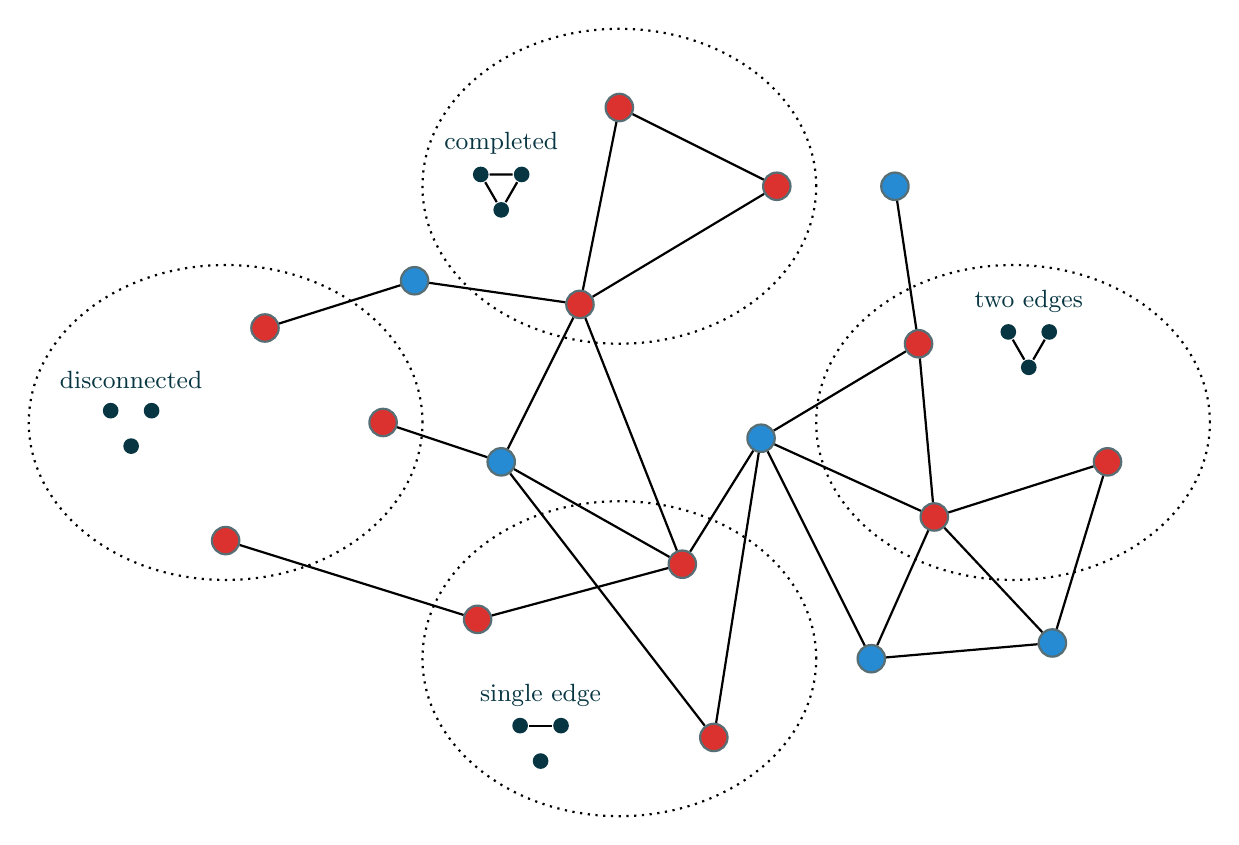
\begin{tikzpicture} [ % 先定义每类点的样式
            thick, >=stealth, scale=1, font=\small,
            plain/.style = {draw=none, text=Solarized-base02},
            point-legend/.style = {circle, inner sep=2pt, fill=Solarized-base02},
            point-red/.style = {circle, inner sep=3.5pt, fill=Solarized-red, draw=Solarized-base01},
            point-blue/.style = {circle, inner sep=3.5pt, fill=Solarized-blue, draw=Solarized-base01}
        ]

        % 宏
        \pgfmathsetmacro{\x}{5}; % 左右椭圆的横坐标
        \pgfmathsetmacro{\y}{3}; % 上下椭圆的横坐标
        \pgfmathsetmacro{\ex}{2.5}; % 椭圆长轴
        \pgfmathsetmacro{\ey}{2}; % 椭圆短轴
        \pgfmathsetmacro{\r}{0.3}; % 等边三角形中心到顶点的距离

        % 椭圆
        \draw [dotted] (-\x,0) ellipse (\ex*1 and \ey);
        \draw [dotted] (0,\y) ellipse (\ex*1 and \ey);
        \draw [dotted] (\x,0) ellipse (\ex*1 and \ey);
        \draw [dotted] (0,-\y) ellipse (\ex*1 and \ey);

        % 蓝色点
        \node [point-blue] (pb1) at (-2.6,1.8) {};
        \node [point-blue] (pb2) at (-1.5,-0.5) {};
        \node [point-blue] (pb3) at (1.8,-0.2) {};
        \node [point-blue] (pb4) at (3.2,-3) {};
        \node [point-blue] (pb5) at (5.5,-2.8) {};
        \node [point-blue] (pb6) at (3.5,3) {};

        % 左 画等边三角形 先确定中心c1 然后依次旋转30、150、270度得到三个顶点
        \path (-6.2,0) coordinate (c1);
        \path (c1) ++(30:\r) coordinate (c11);
        \path (c1) ++(150:\r) coordinate (c12);
        \path (c1) ++(270:\r) coordinate (c13);
        \node [point-legend] at (c11) {};
        \node [point-legend] at (c12) {};
        \node [point-legend] at (c13) {};
        \path (c1) ++(90:\r*1.8) coordinate (c14);
        \node [plain] at (c14) {disconnected};

        \node [point-red] (pr11) at (-4.5,1.2) {};
        \node [point-red] (pr12) at (-3,0) {};
        \node [point-red] (pr13) at (-5,-1.5) {};

        % 上
        \path (-1.5,3) coordinate (c2);
        \path (c2) ++(30:\r) coordinate (c21);
        \path (c2) ++(150:\r) coordinate (c22);
        \path (c2) ++(270:\r) coordinate (c23);
        \node [point-legend] (pl21) at (c21) {};
        \node [point-legend] (pl22) at (c22) {};
        \node [point-legend] (pl23) at (c23) {};
        \path (c2) ++(90:\r*1.8) coordinate (c24);
        \node [plain] at (c24) {completed};
        \draw (pl21) -- (pl22) -- (pl23) -- (pl21);

        \node [point-red] (pr21) at (2,3) {};
        \node [point-red] (pr22) at (0,4) {};
        \node [point-red] (pr23) at (-0.5,1.5) {};
        \draw (pr21) -- (pr22) -- (pr23) -- (pr21);

        % 右
        \path (5.2,1) coordinate (c3);
        \path (c3) ++(30:\r) coordinate (c31);
        \path (c3) ++(150:\r) coordinate (c32);
        \path (c3) ++(270:\r) coordinate (c33);
        \node [point-legend] (pl31) at (c31) {};
        \node [point-legend] (pl32) at (c32) {};
        \node [point-legend] (pl33) at (c33) {};
        \path (c3) ++(90:\r*1.8) coordinate (c34);
        \node [plain] at (c34) {two edges};
        \draw (pl31) -- (pl33) -- (pl32);

        \node [point-red] (pr31) at (3.8,1) {};
        \node [point-red] (pr32) at (4,-1.2) {};
        \node [point-red] (pr33) at (6.2,-0.5) {};
        \draw (pr31) -- (pr32) -- (pr33) -- (pb5);

        % 下
        \path (-1,-4) coordinate (c4);
        \path (c4) ++(30:\r) coordinate (c41);
        \path (c4) ++(150:\r) coordinate (c42);
        \path (c4) ++(270:\r) coordinate (c43);
        \node [point-legend] (pl41) at (c41) {};
        \node [point-legend] (pl42) at (c42) {};
        \node [point-legend] (pl43) at (c43) {};
        \path (c4) ++(90:\r*1.8) coordinate (c44);
        \node [plain] at (c44) {single edge};
        \draw (pl42) -- (pl41);

        \node [point-red] (pr41) at (-1.8,-2.5) {};
        \node [point-red] (pr42) at (0.8,-1.8) {};
        \node [point-red] (pr43) at (1.2,-4) {};
        \draw (pr13) -- (pr41) -- (pr42) -- (pb2) -- (pr43) -- (pb3) -- (pb4) -- (pb5) -- (pr32) -- (pb4);

        % 连线
        \draw (pr11) -- (pb1) -- (pr23) -- (pb2) -- (pr12);
        \draw (pb6) -- (pr31) -- (pb3) -- (pr32);
        \draw (pb3) -- (pr42) -- (pr23);

    \end{tikzpicture}

    \caption{The four different size-3 graphlets that can occur in a simple graph.}
\end{figure}


\end{document}
